%% Copernicus Publications Manuscript Preparation Template for LaTeX Submissions
%% ---------------------------------
%% This template should be used for copernicus.cls
%% The class file and some style files are bundled in the Copernicus Latex Package, which can be downloaded from the different journal webpages.
%% For further assistance please contact Copernicus Publications at: production@copernicus.org
%% https://publications.copernicus.org/for_authors/manuscript_preparation.html


%% Please use the following documentclass and journal abbreviations for preprints and final revised papers.

%% 2-column papers and preprints
\documentclass[amt, manuscript]{copernicus}



%% Journal abbreviations (please use the same for preprints and final revised papers)

%% \usepackage commands included in the copernicus.cls:
%\usepackage[german, english]{babel}
%\usepackage{tabularx}
%\usepackage{cancel}
%\usepackage{multirow}
%\usepackage{supertabular}
%\usepackage{algorithmic}
%\usepackage{algorithm}
%\usepackage{amsthm}
%\usepackage{float}
%\usepackage{subfig}
%\usepackage{rotating}


\begin{document}

\title{TEXT}


% \Author[affil]{given_name}{surname}

\Author[]{}{}
\Author[]{}{}
\Author[]{}{}

\affil[]{ADDRESS}
\affil[]{ADDRESS}

%% The [] brackets identify the author with the corresponding affiliation. 1, 2, 3, etc. should be inserted.

%% If an author is deceased, please mark the respective author name(s) with a dagger, e.g. "\Author[2,$\dag$]{Anton}{Aman}", and add a further "\affil[$\dag$]{deceased, 1 July 2019}".

%% If authors contributed equally, please mark the respective author names with an asterisk, e.g. "\Author[2,*]{Anton}{Aman}" and "\Author[3,*]{Bradley}{Bman}" and add a further affiliation: "\affil[*]{These authors contributed equally to this work.}".


\correspondence{NAME (EMAIL)}

\runningtitle{TEXT}

\runningauthor{TEXT}



\firstpage{1}

\maketitle



\begin{abstract}
TEXT
\end{abstract}


\copyrightstatement{TEXT}


\introduction  %% \introduction[modified heading if necessary]
TEXT
\section{Introduction}

\section{Data and methods}

\subsection{ICI}
%
%t
\begin{table*}[t]
	\label{tab:QRNN_models}	
	\caption{TEXT}
	\begin{tabular}{lrrrr}
		\tophline
		Channel & Frequency 	& Bandwidth  	&NE$\Delta$T	&Polarisation\\
		\middlehline
		I1V&	183.31$\pm$7.00    & 2.0 			& 0.8 		& V\\
		I2V&	183.31$\pm$3.40    & 1.5 			& 0.8 		& V\\
		I3V&	183.31$\pm$2.00    & 1.5 			& 0.8 		& V\\
		I4V&	243.20$\pm$2.50    & 3.0 			& 0.7 		& V\\
		I4H&	243.20$\pm$2.50    & 3.0 			& 0.7 		& H\\
		I5V&	325.15$\pm$9.50    & 3.0 			& 1.2 		& V\\
		I6V&	325.15$\pm$3.50    & 2.4 			& 1.3 		& V\\
		I6V&	325.15$\pm$1.50    & 1.6 			& 1.5 		& V\\
		I8V&	448.00$\pm$7.20    & 3.0 			& 1.4 		& V\\
		I9V&	448.00$\pm$3.00    & 2.0 			& 1.6 		& V\\
		I10V&	448.00$\pm$1.40    & 1.2 			& 2.0 		& V\\
		I11V&	664.00$\pm$4.20    & 5.0 			& 1.6 		& V\\
		I11H&	664.00$\pm$4.20    & 5.0 			& 1.6 		& H\\		
		\bottomhline
	\end{tabular}
	\begin{tabular}{lrrrr}
		\tophline
		Channel & Frequency 	& Bandwidth  	&NE$\Delta$T	&Polarisation\\
		\middlehline
		MWI-14&	183.31$\pm$7.00    & 2.0 			& 1.3 		& V\\
		MWI-15&	183.31$\pm$6.10    & 1.5 			& 1.2 		& V\\
		MWI-16&	183.31$\pm$4.90    & 1.5 			& 1.2 		& V\\
		MWI-16&	183.31$\pm$3.40    & 1.5 			& 1.2 		& V\\
		MWI-16&	183.31$\pm$2.00    & 1.5 			& 1.3 		& V\\	
		\bottomhline
	\end{tabular}
	\belowtable{} % Table Footnotes
\end{table*}
Ice Cloud Imager (ICI) is a new EPS-SG (EUMETSAT Polar System - Second Generation) sensor that will observe  Earth using submillimeter-wave (sub-mm) frequency range. The main objective of ICI is measure ice cloud properties and improve the representation of clouds in regional and global models. ICI is a conically scanning millimetre/sub-millimetre radiometer which will measure 13 frequencies from 183 GHz up to 664 GHz. Channels with centre frequencies 183.31, 325.15 and 448.0\,GHz are centered on water vapor absorption lines, and measure vertical polarization. While other channels around 243.0 and 664.0\,GHz are ``window channels'' and receive both vertical and horizontal polarization. 
In addition to ICI, the EPS-SG satellite will also have Microwave Imager (MWI) onboard. MWI will measure frequencies from 18.7 GHz up to 183\,GHz and provide data continuity to the existing microwave imager measurements. The common 183\,GHz channels among the two instruments shall allow cross-calibration between the two instruments. The channel configurations for ICI and MWI (only 183\,GHz) are provided in Table~\ref{tab:ICI_MWI_configuration}.

\subsection{ICI simulations}
%
**** Some parts copied directly from AWS report *****

The satellite observations for all ICI channels are simulated with the Atmospheric Radiative Transfer Simulator (ARTS, (ARTS, \citet{eriksson:arts2:11,buehler:artst:18})version. The simulations include TB from five ICI channels around 183\,GHz, 243\,GHz, 325\,GHz, 448\,GHz and 664\,GHz. 

The absorption model takes into account the effect from nitrogen \citep{pwr:93}, oxygen \citep{pwr:93} and water vapour \citep{ellison2007permittivity}. LWC is taken from ERA-Interim and is assumed to be totally absorbing. In the
mapping of CloudSat reflectivities to RWC and IWC a total separation between
liquid and ice phase is assumed. All scattering hydrometeors at temperatures
above 0$^\circ$C are assumed to be rain, and all below 0$^\circ$C are assumed
to be ice hydrometeors. For RWC the particle size distribution of \citet{abel2012improved} is applied. The PSD of IWC follows the basic formulation applied in DARDAR (\verb http://www.icare.univ-lille1.fr/projects/dardar), using latest parameter values (i.e.\ $\alpha$ and $\beta$) as given by
\citet{amt-12-2819-2019}. This PSD can be considered as a ``two moment''
scheme, but is here applied in a one moment manner by setting $N_0^*$ (as a
function of temperature) following Table~5 of \citet{delanoe2014normalized},
and letting the radar reflectivity set the remaining moment.
Single scattering data are taken from \citet{eriksson:agene:18}. For ice
hydrometeors, three habits are applied: Perpendicular 3-bullet rosette, Large
plate aggregate and Large column aggregate. In the last two cases, the
aggregates are complemented with single crystal data to also cover smaller
sizes. These data describe particles assumed to have a totally random
orientation. To apply oriented particles is much more computationally costly
and could not be accommodated inside the study. The land emissivity was taken from TELSEM \citep{aires2011tool} and the Ocean/water from TESSEM \citep{prigent2017sea}. For each atmopsheric case, both ''clear-sky'' and ``all-sky'' calculations were performed. In the former, all impact of all hydrometeors were set to zero, while in the latter, IWC and RWC derived from CloudSat reflectivities and LWC from ERA-Interim were taken into account. Both sets of calculations were made by ARTS's interface to the RT4 solver \citep{evans1995microwavec}. To avoid a possible bias between clear-sky and all-sky for insignificant hydrometeor contents, the same ``scattering solver'' was used for both calculations. The first two elements of the
Stokes vector were calculated.

\subsection{Simulation dataset}
%
Using the simulation setup described in previous section, Cloudsat profiles during August 2015 were randomly selected to generate 200\,000 cases for each ICI frequency. The input data were restricted between $60^{\degree}$S to $60^{\degree}$N, and surface is below 500\,m. Both clear-sky and all-sky scenarios were simulated, and no differentiation was made between the observations over ocean/sea and land. It is also assumed that all simulations are remapped to a common foorprint. 

**** show any comparsion to ATMS? or AWS channels ? ****

\subsection{QRNN}
%
The neural network training is a process of learning to predict the outputs {$y_i$} from inputs {$x_i$} through a series of learnable transformations. While training, neural networks seek to minimise the model error through a loss function. The choice of the loss function depends on the predictive problem. When a neural network is trained to minimise the mean of the quantile loss function to predict the quantiles of the distribution, it is called a Quantile Regression Neural Network (QRNN). 

 
\subsubsection{Model selection}
%
\label{model_selection}
A high performing QRNN model requires tuning of multiple hyper-parameters. These parameters determine the structure and the training set-up of the neural network. Several of these hyper-parameters are non-learnable, and must be defined before beginning of every training. Grid search is one of the most often employed techniques for hyper-paramter tuning. In grid search, different combinations of hyperparamters are selected and for each, the model performance is evaluated. The model architecture with the best performance is selected. The model evaluation metrics employed in this article are described in the next section. 

For the structural parameters, the grid search is performed to determine the number of neurons (width) and hidden layers (depth). The model is trained for multiple values of layer widths and hidden layers, and the best configuration is selected by evaluating the predictions over the validation set. Similarly, the training process is optimized by performing a grid search different training parameters such as : batch size, learning rate, number of epochs, decay. The best performing hyperparameter configurations for a particular training set need not be same for other datasets. Therefore for each QRNN model used in this article the hyperparameters were tuned distinctly. 

\subsubsection{Evaluation metrics}

Quantile loss function

CRPS


\section{Cloud correction in ICI 183 GHz channels}
%
\subsection{Training data}
%
Out of the 200\,000 ICI channel simulations, 150\,000 cases are randomly picked to form the training set. The rest are used for testing. In the training set, 90\% of the data is randomly selected to form the training set, while the other 10\% form the \textit{testing-during-training} database. ARTS simulations are noise free, so to incorporate the satellite measurement uncertainties, gaussian noise is added to the input training data according to the channel NE$\Delta$T. The target training data is kept noise free. In order to build a robust learning network, random noise is added to the inputs at each training iteration. This exposes the model to a different datasets during the entire training process and avoids the memorisation of training samples. The input data is also normalized with mean and standard deviation.

\subsection{Training}
%
%t
\begin{table}[t]
\label{tab:QRNN_models}	
\caption{TEXT}
\begin{tabular}{lll}
\tophline
QRNN model & Training inputs & Target \\
\middlehline
QRNN-simple & I1V, I5V, I6V, I7V, I8V, I9V, I10V, I11V & I1V\\
			& I2V, I5V, I6V, I7V, I8V, I9V, I10V, I11V & I2V\\
			& I3V, I5V, I6V, I7V, I8V, I9V, I10V, I11V & I3V\\
QRNN-all    & I1V, I2V, I3V, I5V, I6V, I7V, I8V, I9V, I10V, I11V & I1V\\	
			& I1V, I2V, I3V, I5V, I6V, I7V, I8V, I9V, I10V, I11V & I2V\\	
			& I1V, I2V, I3V, I5V, I6V, I7V, I8V, I9V, I10V, I11V & I3V\\
QRNN-mwi	& MWI-15, I5V, I6V, I7V, I8V, I9V, I10V, I11V & MWI-15\\	
			& MWI-16, I5V, I6V, I7V, I8V, I9V, I10V, I11V & MWI-16\\			
\bottomhline
\end{tabular}
\belowtable{} % Table Footnotes
\end{table}
To investigate the performance of training inputs, two QRNN models with different set of training inputs are analysed. In both models, the training set combines data from 183\,GHz, 325 GHz, 448\,GHz and 664\,GHz to predict cloud corrected observations for the target 183\,GHz channel.

In the first model, the training set includes the target 183\,GHz channel and the sub-mm channels. For example, to train for channel I1V, the input channels are I1V, I5V , I6V, I7V, I8V, I9V, I10V, I11V. A separate QRNN model is trained for each of the 183\,GHz channels. We shall refer this QRNN model as ``QRNN-simple''. 

In the second QRNN model, we sugest to use all three 183\,GHz channels concurrently  with the other sub-mm channels. In this case, although the input training parameters are same for all channels, QRNN needs to be trained separately each 183\,GHz channel. Further in text, we refer this model as ``QRNN-all''. Table~\ref{tab:QRNN_models} summarises the two QRNN models. 

As described in section \ref{model_selection}, a grid search was implemented to select the best performing hyperparamters. The mean quantile loss and CRPS for different layer width and hidden layer configurations are shown in Fig\ref{fig:model_selection}. The results are for QRNN-simple with I3V as target channel. Increasing the complexity of the network by increasing the layer-width and depth has a positive impact on performance. However for four hidden layers, increasing the number of neurons beyond 128 has no significant impact on the performance. On basis of these results, a neural network with four hidden layers and 128 neurons in each layer was selected for QRNN-simple. 

For the optimising the training paramters, a customised  learning rate scheduler was implemented. The initial learning rate was reset after a certain number of epochs.  We started the training process with a initial learning rate of 0.1, and decreased it by a factor of 10 after 100 epochs. The best neural network performance was obtained when the network was trained three times with a new initial learning rate. For each training  if the validation loss remained unchanged till 6 training epochs, the learning rate was reduced by a factor of 2. We did not optimise the type of activation function and batch size. Rectified Linear Unit (ReLU) was used as the activation function  and the batch size was set to 128 samples for all QRNN models. 
For QRNN-all a grid search (results not shown) over width and depth and learning rates resulted in similar performance, and an identical neural network was selected.

\begin{figure}[t]
	\centering
	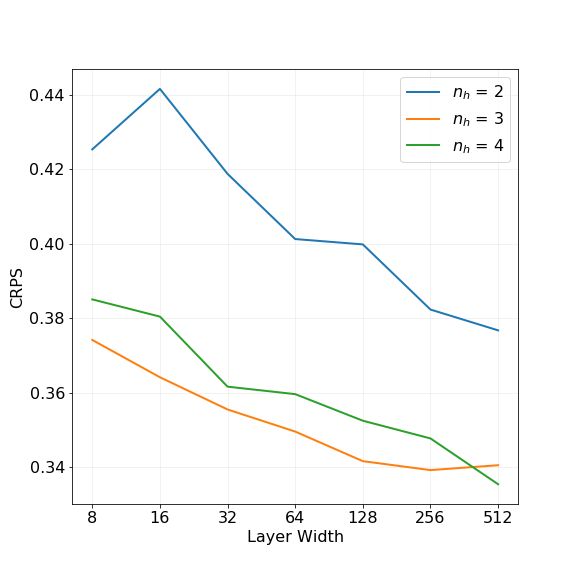
\includegraphics[height=57mm]{Figures/CRPS.png} 
	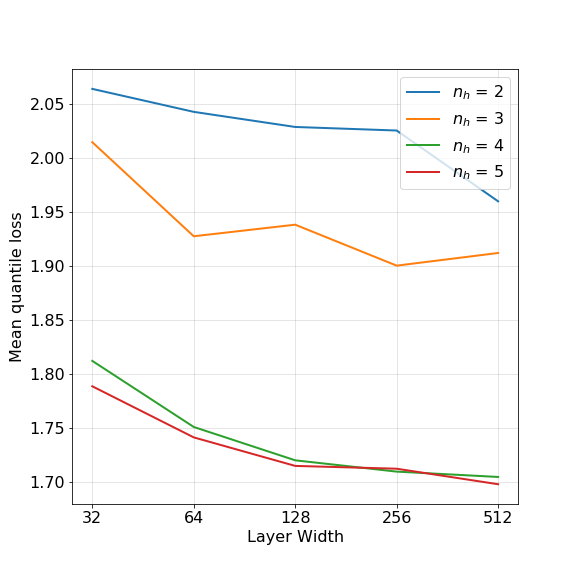
\includegraphics[height=57mm]{Figures/quantile_loss.png}
	\caption{}
	\label{fig:}	
\end{figure}

\subsection{Prediction results}
%
%f 
\begin{figure}[t]
	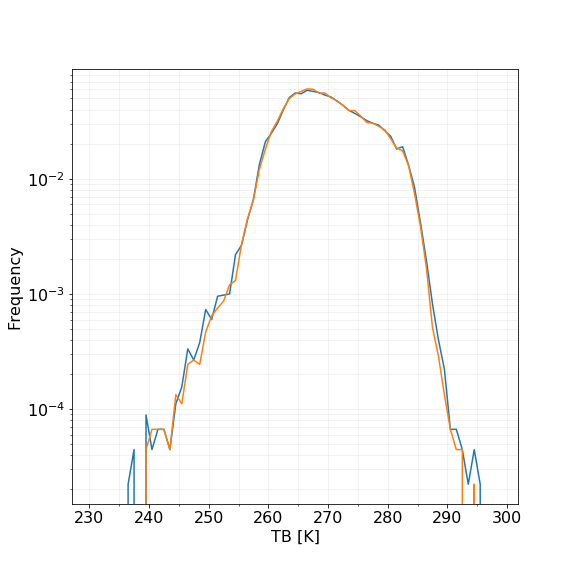
\includegraphics[height=57mm]{Figures/PDF_I1V_single.png} 
	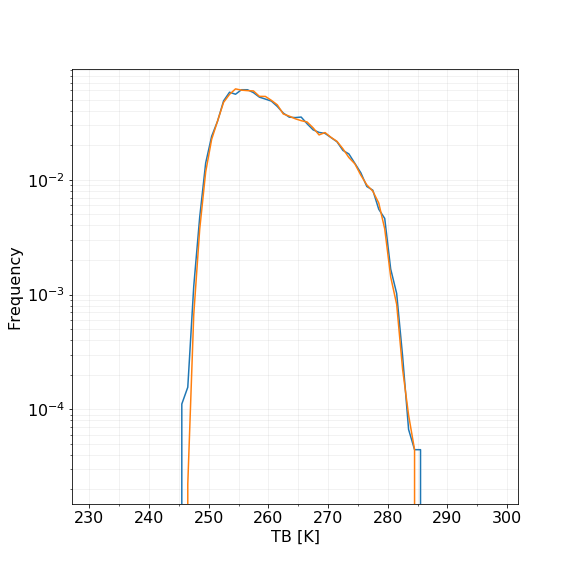
\includegraphics[height=57mm]{Figures/PDF_I2V_single.png}
	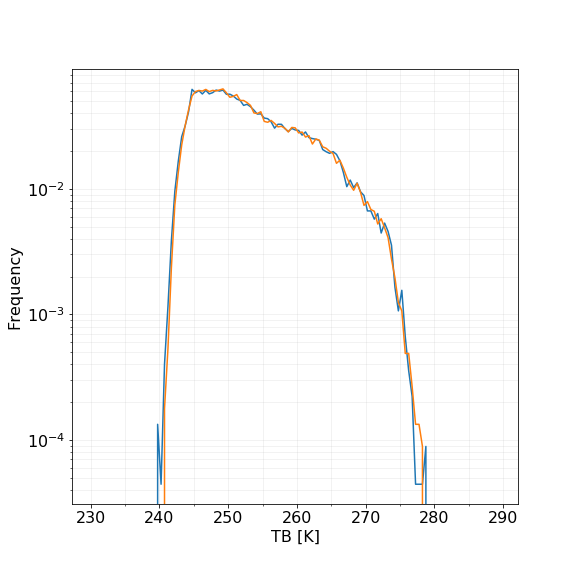
\includegraphics[height=57mm]{Figures/PDF_I3V_single.png} 
	\caption{PDF}
	\label{fig:PDF_predictions}	
\end{figure}
%f 
\begin{figure}[t]
	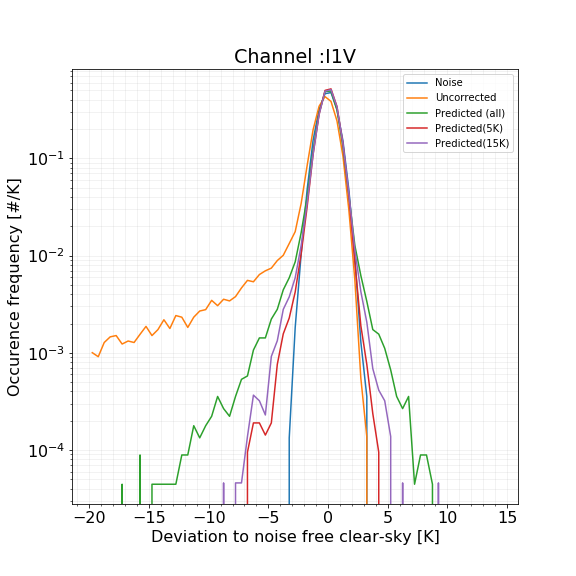
\includegraphics[height=57mm]{Figures/ICI_I1V_single.png} 
	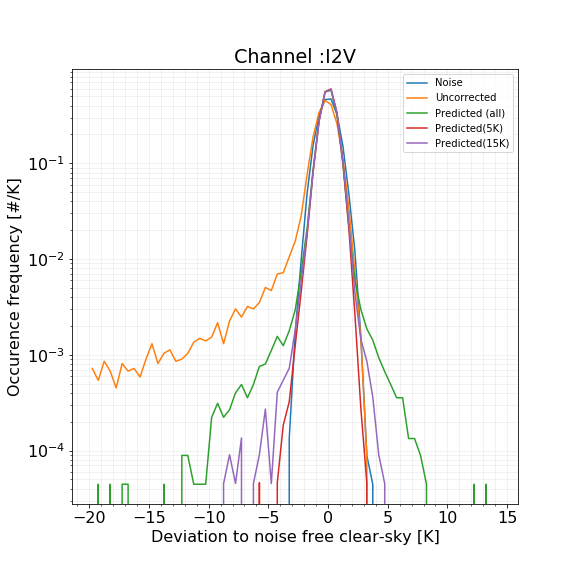
\includegraphics[height=57mm]{Figures/ICI_I2V_single.png}
	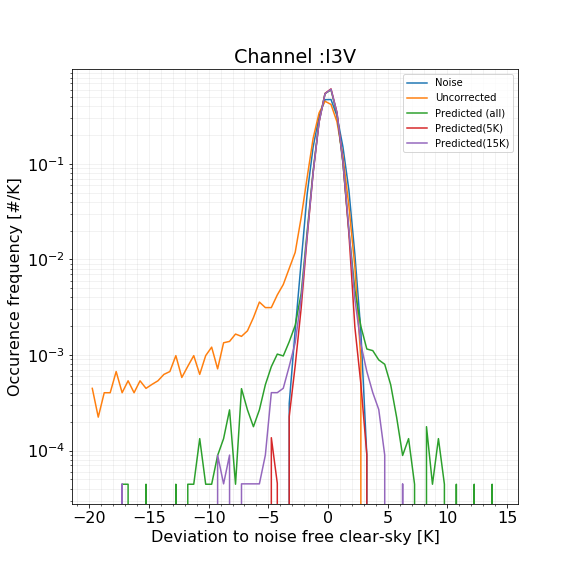
\includegraphics[height=57mm]{Figures/ICI_I3V_single.png} 
	\caption{Error distributions}
	\label{fig:error_distributions}	
\end{figure}

%t
\begin{table}[t]
	\caption{I1V}
	\label{tab:I1V_statistics}
	\begin{tabular}{lrrrrrr}
		\tophline
		&&& \multicolumn{2}{c}{QRNN-simple} & \multicolumn{2}{c}{QRNN-all}\\
		&   noise &   uncorrected &   corrected(all) &   corrected(filtered) & corrected(all) &   corrected(filtered) \\
		\middlehline
		bias     &   -0.00 &         -1.90 &           -0.03 &                 0.00 & -0.01 &                 0.01 \\
		mae      &    0.64 &          2.35 &            0.69 &                 0.60 & 0.66 &                 0.58\\
		std      &    0.80 &          8.92 &            1.05 &                 0.78 &  0.96 &                 0.75\\
		skewness &   -0.01 &         -7.99 &           -1.24 &                -0.44 & -0.39 &                -0.32\\
		rejected &    	 - &          - &            - &                 6.40 & - &                 6.42 \\
		\bottomhline
	\end{tabular}
	\belowtable{} % Table Footnotes
\end{table}
%t
\begin{table}[t]
	\caption{I2V}
	\label{tab:I2V_statistics}
	\begin{tabular}{lrrrrrr}
		\tophline
		&&& \multicolumn{2}{c}{QRNN-simple} & \multicolumn{2}{c}{QRNN-all}\\
		&   noise &   uncorrected &   corrected(all) &   corrected(filtered) & corrected(all) &   corrected(filtered) \\
		\middlehline
		bias     &   -0.00 &         -1.05 &            0.02 &                 0.03&  0.02&   0.03\\
		mae      &    0.64 &          1.54 &            0.56 &                 0.50&  0.46&   0.42\\
		std      &    0.80 &          5.98 &            0.86 &                 0.64&  0.70&   0.53\\
		skewness &    0.02 &        -10.64 &           -2.25 &                -0.22& -1.67&  -0.25\\
		rejected &    - &          - &            - &                 3.70&  - &   3.67\\
		\bottomhline
	\end{tabular}
	\belowtable{} % Table Footnotes
\end{table}

%t
\begin{table}[t]
	\caption{I3V}
	\label{tab:I3V_statistics}
	\begin{tabular}{lrrrrrr}
		\tophline
		&&& \multicolumn{2}{c}{QRNN-simple} & \multicolumn{2}{c}{QRNN-all}\\
		&   noise &   uncorrected &   corrected(all) &   corrected(filtered) & corrected(all) &   corrected(filtered) \\
		\middlehline
		bias     &   0.00 &         -0.63 &            0.02 &                 0.02& 0.04 &                 0.04 \\
		mae      &    0.64 &          1.14 &            0.54 &                 0.50&0.48 &                 0.44 \\
		std      &    0.80 &          4.26 &            0.80 &                 0.64&0.71 &                 0.56 \\
		skewness &   0.00 &        -13.26 &           -1.40 &                -0.16&-1.41 &                -0.11 \\
		rejected &    - &          - &           - &                 2.18&- &                 2.18 \\
		\bottomhline
	\end{tabular}
	\belowtable{} % Table Footnotes
\end{table}
QRNN predictions are estimates of the posterior distribution over different quantiles: $x_{\tau}$, for median, $\pm 1\sigma$, $\pm 2 \sigma$ and  $\pm 3 \sigma$ ($\tau$ = 0.002, 0.03, 0.16, 0.5, 0.84, 0.97, 0.998). The median of the posterior distribution is assumed to be the best estimate for the predicted clear-sky value. The prediction error is calculated as the deviation to the corresponding noise-free clear-sky value. We calculate the mean bias, mean absolute error and standard deviation of the errors. The asymmetry of the distributions around their mean is also calculated through the measure of skewness. In the following sections, we describe the performance of the two QRNN models.

The distributions of the predicted clear-sky values and the clear-sky simulations from QRNN-single are shown in Fig~\ref{fig:PDF_predictions}. The three figures correspond to channels: I1V, I2V and I3V. These results show that the clear-sky values predicted by QRNN-single have a very good match for the peak of the distributions, but a slight mismatch is evident towards the tails, where QRNN seems to predict slightly colder/warmer TBs. 

Fig~\ref{fig:error_distributions} shows the error distributions of the uncorrected measurements and predicted clear-sky TBs for all three channels. Distribution of noise is also plotted for reference.  The error metrics corresponding to these results are provided in Table~\ref{tab:I1V_statistics} - Table~\ref{tab:I3V_statistics}. Without any cloud impact, the error distributions should follow a Gaussian distribution, however the presence of clouds leads to a TB reduction, and introduces a high negative bias. Among the three channels, I1V has the highest cloud impact and I3V has the least. The bias in I1V measurements is -1.89\,K compared to only -0.55\,K in I3V. After correction, the cloud impact is reduced and the resulting error distributions are symmetric with low bias. The predictions and the observations have a good agreement for the main peak of the distribution, albeit the prediction errors have a sharper peak and a larger spread. The larger spread indicates few cases which are under-/over corrected. If all the cases with correction greater than 15\,K are excluded, only a fraction of the total cases are removed but the  the variability in predictions errors reduces significantly. This indicates low accuracy of QRNN predictions for cases with high cloud impact.

Compared to channel I1V, the performance of QRNN model is slighly better for I2V and I3V.   

The error metrics from QRNN-all are also shown in the last columns of Table~\ref{tab:I1V_statistics} - Table~\ref{tab:I3V_statistics}. As expected, using additional 183\,GHz channels improves the accuracy of the predictions slightly.  

**** add QRNN-all results ****

\subsection{Uncertainty quantification}
%
%f 
\begin{figure}[t]
	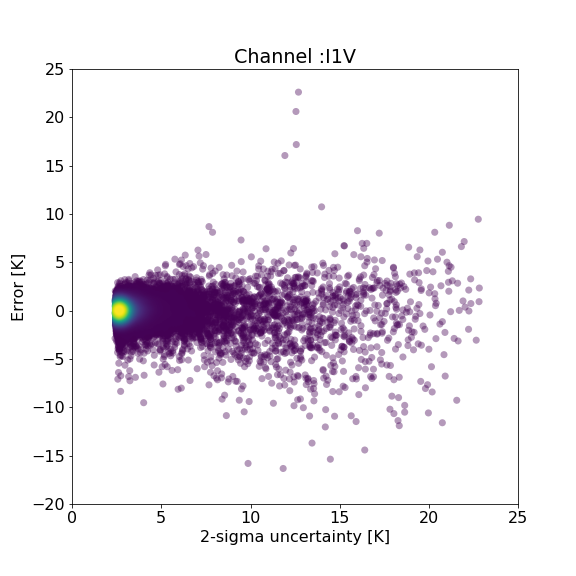
\includegraphics[height=57mm]{Figures/scatter_uncertainty_single_I1V.png} 
	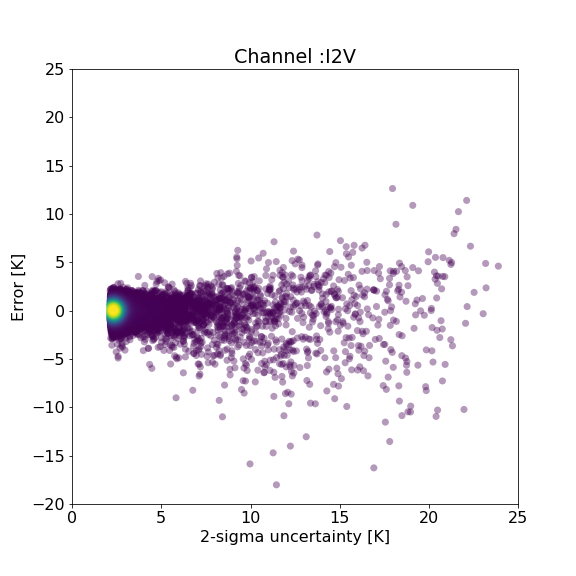
\includegraphics[height=57mm]{Figures/scatter_uncertainty_single_I2V.png}
	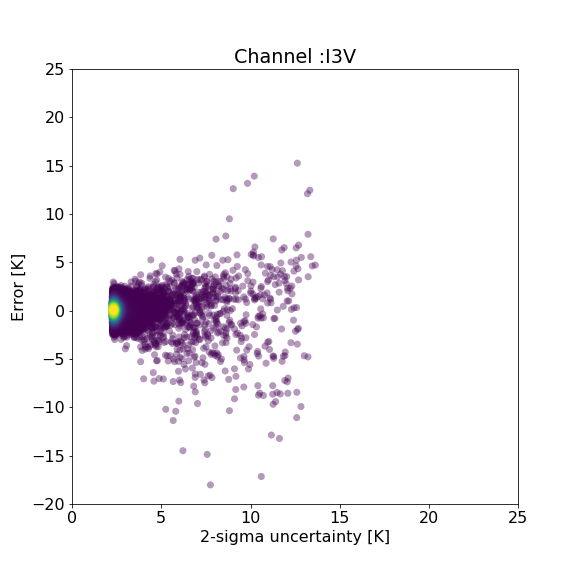
\includegraphics[height=57mm]{Figures/scatter_uncertainty_single_I3V.png} \\
	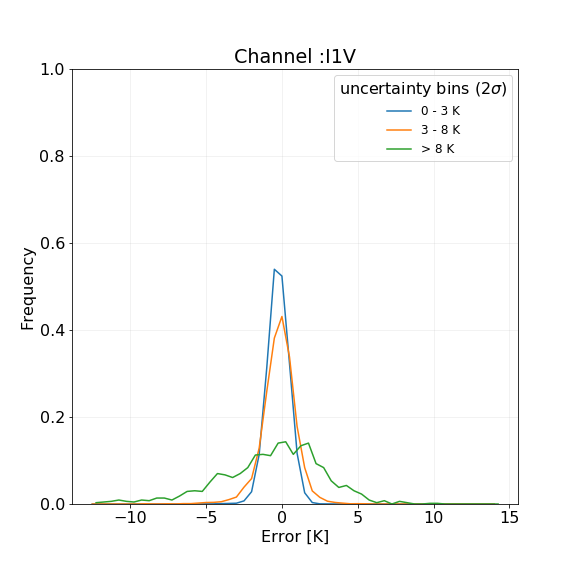
\includegraphics[height=57mm]{Figures/Frequency_uncertainty_bins_I1V_single.png} 
	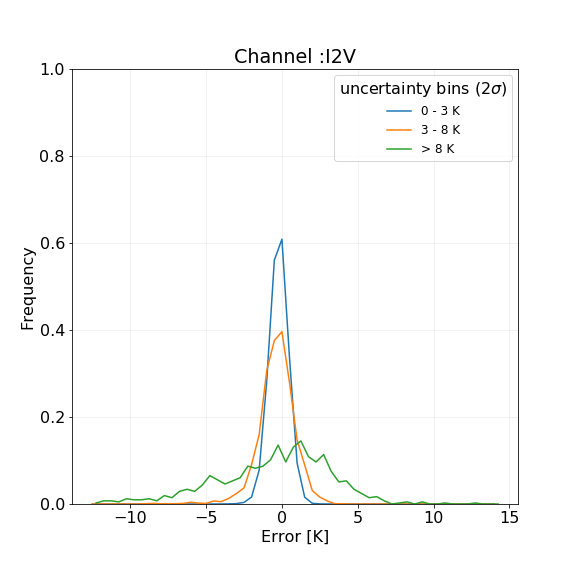
\includegraphics[height=57mm]{Figures/Frequency_uncertainty_bins_I2V_single.png}
	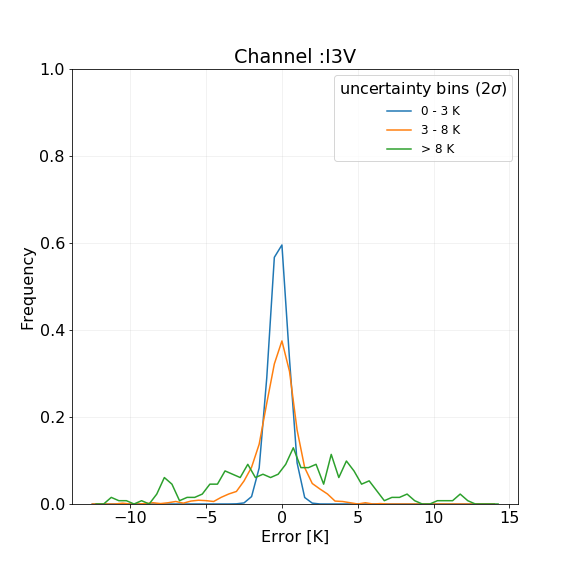
\includegraphics[height=57mm]{Figures/Frequency_uncertainty_bins_I3V_single.png}
	\\	
	\caption{}
	\label{fig:error_distributions}	
\end{figure}
The biggest advantage of using QRNN is estimation of case-specific uncertainties. The quantiles can be used to construct a probability distribution of the
predictions in contrast to other correction approaches which give out only point estimates. In all QRNN models presented in this article, we estimate the conditional
quantiles for median, $\pm 1\sigma$, $\pm 2\sigma$, and $\pm 3\sigma$. The
predictions for each quantile are used to construct the confidence intervals.
The confidence interval for each point estimate quantifies its uncertainty. For example, the predicted quantiles for $\pm 2 \sigma$ implies that there is  94\% probability that the true value will lie between the range.

Fig~\ref{fig:uncertainty_scatter} shows the scatter plot between the error and uncertainty. The error distributions for all three channels are centered around zero, however the uncertainty in predictions for I1V and I2V are higher than I3V. An increase in the spread with increasing uncertainty is evident in all three. As the errors increase, the spread is mostly symmetric around x-axis but for high uncertainty values, negative errors occur more frequently. This suggests that predictions for cases high cloud impact are associated with high uncertainty. The lower panel in the same figure, shows the errors when plotted as distributions over different uncertainty bins. Apart from few individual variations, all three channels follow the trend of increasing uncertainty with decreasing accuracy, suggesting that QRNN is successful in providing well calibrated probabilistic predictions of the posterior distribution. 

%Fig~\ref{fig:uncertainty_estimate} shows the prediction uncertainties for randomly chosen 2000 cases. A large spread in the plot indicates a high case-to-case variability of the uncertainty. 


%To inspect if the predictions follow a normal distribution, we evaluate the length of confidence intervals from the median. Figure~\ref{fig:prediction_uncertainty} shows the prediction uncertainty in AWS-34 (four channel option). The uncertainty with respect to the median for 1000 randomly selected cases is shown. The red line represents the uncertainty in a hypothetical Gaussian distribution of $270\pm0.62$\,K. If the underlying distribution is Gaussian, the prediction uncertainty should be symmetric around the median, and the uncertainties should be equally spaced for $1\sigma$, $2\sigma$ and so on. The predictions from our QRNN model seem to be symmetric around the median for the 94\% confidence interval ($\pm 2 \sigma$). The figure also shows that the uncertainties for all 1000 random cases are concentrated along a narrow width, thus suggesting that the case to case variability of the uncertainty is low. A similar uncertainty quantification for other 183\,GHz channels also gives similar results. 

%f
%\begin{figure}[t]
%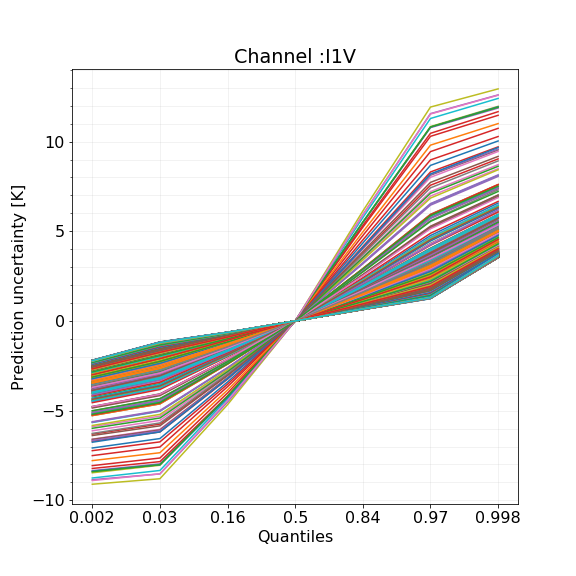
\includegraphics[height=57mm]{Figures/uncertainty_single_I1V.png} 
%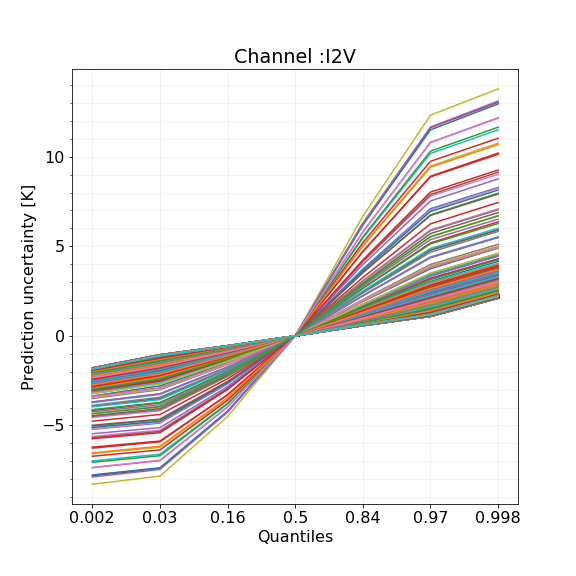
\includegraphics[height=57mm]{Figures/uncertainty_single_I2V.png}
%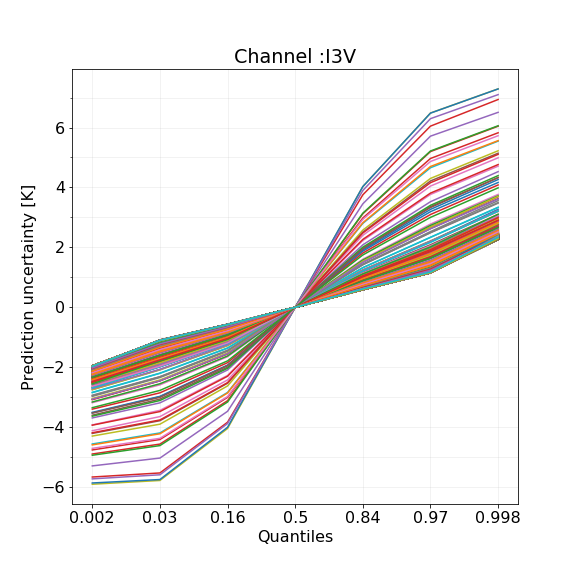
\includegraphics[height=57mm]{Figures/uncertainty_single_I3V.png} 
%\caption{}
%\label{fig:}
%\end{figure}




\section{Special case of using only 325\,GHz for cloud correction}

\subsection{Data}
24 monochromatic frequencies were used so that each channel could be represented
with sufficient accuracy. The simulations were generated for sensor viewing angles from
$0^{\circ}$ to $45^{\circ}$, but all the results described here are based on nadir viewing angle.


\subsection{Training}

\subsection{Prediction results}


\conclusions  %% \conclusions[modified heading if necessary]


%% The following commands are for the statements about the availability of data sets and/or software code corresponding to the manuscript.
%% It is strongly recommended to make use of these sections in case data sets and/or software code have been part of your research the article is based on.

\codeavailability{TEXT} %% use this section when having only software code available


\dataavailability{TEXT} %% use this section when having only data sets available


\codedataavailability{TEXT} %% use this section when having data sets and software code available


\sampleavailability{TEXT} %% use this section when having geoscientific samples available


\videosupplement{TEXT} %% use this section when having video supplements available


\appendix
\section{}    %% Appendix A

\subsection{}     %% Appendix A1, A2, etc.


\noappendix       %% use this to mark the end of the appendix section. Otherwise the figures might be numbered incorrectly (e.g. 10 instead of 1).

%% Regarding figures and tables in appendices, the following two options are possible depending on your general handling of figures and tables in the manuscript environment:

%% Option 1: If you sorted all figures and tables into the sections of the text, please also sort the appendix figures and appendix tables into the respective appendix sections.
%% They will be correctly named automatically.

%% Option 2: If you put all figures after the reference list, please insert appendix tables and figures after the normal tables and figures.
%% To rename them correctly to A1, A2, etc., please add the following commands in front of them:

\appendixfigures  %% needs to be added in front of appendix figures

\appendixtables   %% needs to be added in front of appendix tables

%% Please add \clearpage between each table and/or figure. Further guidelines on figures and tables can be found below.



\authorcontribution{TEXT} %% this section is mandatory

\competinginterests{TEXT} %% this section is mandatory even if you declare that no competing interests are present

\disclaimer{TEXT} %% optional section

\begin{acknowledgements}
TEXT
\end{acknowledgements}




%% REFERENCES


 \bibliographystyle{copernicus}
 \bibliography{example.bib}

\end{document}
